\documentclass[12pt,a4paper]{article}
\usepackage[utf8]{inputenc}
\usepackage[spanish]{babel}
\usepackage{amsmath}
\usepackage{amsfonts}
\usepackage{amssymb}
\usepackage{makeidx}
\usepackage{graphicx}
\usepackage{url}
\usepackage{lmodern}
\usepackage{kpfonts}
\usepackage{fourier}
\usepackage[left=2cm,right=2cm,top=2cm,bottom=2cm]{geometry}
\author{Rodriguez Lopez Francisco Javier}
\begin{document}

\begin{center}
\LARGE \textbf{Universidad Politecnica de la Zona Metropoilitana de Guadalajara\\}



\includegraphics[width=7cm]{UpzmgD.png}  

\LARGE \textbf{Tiristores en Convertidores CA-CD y CA-CA}\\
\vspace{2cm}
\large \textbf{Nombre: Rodriguez Lopez Francisco Javier.\\
\vspace{0.5cm} Matricula: 18311804.\\
\vspace{0.5cm} Carrera: Ingenieria en Mecatronica.\\
\vspace{0.5cm} Materia: Sistemas Electronicos de Interfaz.\\
\vspace{0.5cm} Curso: septiembre-diciembre del 2019.\\
\vspace{0.5cm} Docente: Moran Garabito Carlos Enrique.}


\vspace{6cm}
\small \textbf{24 de Septiembre del 2019}
\end{center}

\section{Tiristores:}
El tiristor, es un componente semiconductor, esto da a entender que trabaja de igual forma que un diodo rectificador, siendo este, un paro de corriente por el circuito que maneje, este tiene que ver mucho la temperatura que lo acompañe, ya que el aparte de servir como semiconductor, tambien puede servir como un aislante, el cual se emplea por la potencia electrica que este tenga el control, esto lo caracteriza de ser un dispositivo inidireccional, o bidireccional.

\subsection{CA-CD:}

Para poder hacer una controlacion de un circuito de convertidor, de CA-CD, se tiene en cuenta que se ocupa de tiristores, puesto que estos pueden controlar el angulo de disparo, y de ello depender como se manejara la onda recibida, siendo esto el control de todo el convertidor.
Como su nombre lo explica, conlleva de muchos factores ya que este circuito, sustituye los diodos, por los SCRs, de este el angulo es un predominante a tener en cuenta, esto determinado por las fases que cruza la onda, y este depende del angulo que tenga la carga.\\

\begin{figure}[hbtp]
\caption{Circuito CA-CD Controlado}
\centering
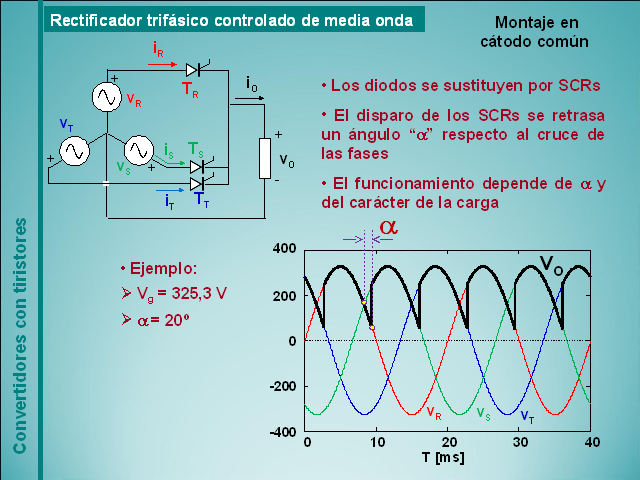
\includegraphics[width=8cm]{img1.png}
\end{figure}

Como se aprecia en el circuito en el se ve el tiristor en la parte superior, en donde este es el que controla la onda que se muestra de igual manera en la imagen. Para poder realizar la operacion hay que tener en cuenta lo siguiente.

\emph{fourier}
$$ Vo_{med}= \frac{3}{2\pi} \int_\frac{2x/6}* cos(w_{red}* t)* d(w_{red}* t= \frac{3}{\pi}V_{g}* sin(\frac{\pi}{3}* cos a $$

Esta formula nos describe, la tension media de salida todo esto en funcion del angulo de disparo, que tiene el tiristor en retraso. Se puede ver que se maneja tanto coseno, como seno, siendo coseno uan parte que trabajara con la fuente red, respecto al tiempo, trabajando el voltaje necesario para sobrepasar el voltaje del tiristor y siendo seno el participe de pi entre 3 multiplicado por el conseno del angulo.\\

Nos da a entender que coseno es el que trabaja con el tiristor para que este tenga un control y una face en media onda.\\
si hay fases la formula utilizada es:
\emph{fourier}
$$ Vo_{med}= \frac{P}{\pi} V_{g}* sin(\frac{\pi}{p})* cos a $$

Siempre hay que tener en cuenta una cosa antes de realizar cualquier operacion, esta formula no sirve, cuando la tension se queda en cero.

Para tener mas en cuenta esto, se trabaja con el catodo comun, de dicha funcion, o en este caso dicho circuito, para la genercion de la onda, y del convertido de la fuente CA-CD. Si la generacion de la carga es muy inductiva, y tiene retrasos moderados, se debe de tomar en cuenta algo, la onda de generacion completa se acortara a la mitad, y de ello su tiempo de caida sera mas rapido, siendo el participe del circuito que genere el disparo, con el calculo que se dio en la parte de arriba.\\

Si el angulo es de 90°, entonces el voltaje de la tension media se pasara a 0, esto por que tiene un tope, por nede no habar potencia activa en la correinte de fase, si el angulo llegar a ser mayor, entonces el voltaje pasara a ser negativo, por lo que sus traspaso, de corriente estaran mas elevados de lo que normalmente deberian de estar. Siendo que la carga del crcuito tenga que estar activa.\\

Cuando la carga es muy inductiva, en un angulo determinado que no traspase los 90°, el circuito y el tiristor operan como un rectificador normal, siendo este la funcion que normalmente cumpliria.\\ 

Pero en caso de que este sobrepase los 90°, su funcion sera diferente interfiriendo mucho en la potencia, ya que trabajara como inversor, y descargara dicho circuito.\\

En otro caso peculiar, si el angulo de disparo es menor a 30°, el voltaje de inicio pasara a ser un carga muy inductiva, para el circuito, llegando a este punto, si se trata con una tension muy inductiva, los tiristores lo que haran, seran llevar su corriente a cero.\\

En cuestion, el calculo de la tension media de salida de carga resistiva pura en fucion del angulo de disparo, respecto al retraso queda:

\emph{fourier}
$$ Vo_{med}= \frac{3}{2\pi} \int_\pi V_{g}* sin(w_{red}* t)* d(w_{red}* t)= \frac{3}{2\pi} V_{g}* (1+ sin(\frac{\pi}{3}-a)) $$

En este caso el angulo que maneje, ya sea este de 45°, o 120°, no afecta este por la tension con carga pura resistiva, ya sea el angulo de disparo, el corde y adecuado, para hacer que el tiristor pase la corriente de forma buena, se debe de tomar en cuenta, que entre mas grande sea el angulo, en este caso, la onda se acortara a tal grado de hacerla un pico muy pequeño, el cual va de la funcion paro de corriente, subida de la onda y caida repentina y en cuestion el angulo que se maneje, sera menor al del angulo menor.

\subsection{CA-CA:}

Para estos casos, el circuto es un poco mas complejo de hacer, pero debemos de tomar en cuenta, que estamos trabajando, con el mismo conversor de fuente, siendo esta la misma, lo que tratamos aqui es controlar el voltaje, que se pasara, y de esta forma, el tiristor cumple su fucnion, regulando, y pasando de ser un simple rectificador  aun aislante.\\

El voltaje inicial se calcula de la siguiente manera:
\emph{fourier}
$$ Vo= V_{P0}- V_{N0} $$

Sinedo este primordial para todos, ya que de esto deriva toda la carga de las fuentes, que se estaran trabajando.

Si el angulo de disparo, respecto a la carga es menor a 60°, se puede utilizar una formula que describa el voltaje medio de este.
\emph{fourier}
$$ Vo_{med}= 2* \frac{3}{\pi}Vo* sin(\frac{\pi}{3})* cos(a) $$

En este caso, las ondas generadas a partir del buen uso de la formula conllevado por el voltaje de inicio, y la carga ya sea esta muy inductiva, generaran ondas de igual forma acortando la onda completa a la mitad, pero siendo estas directas, y solo trabajando en la parte de arriba.\\
En este caso, tambien pasa lo mismo, puesto que entre mas angulo tenga su voltaje medio, pasara a ser de menor valor, ya que la rectficacion, pasara a ser solamente de la parte de arriba, a trabajar con una parte del inversor, y otra de la misma rectificacion.\\
Mientras mas grande es el angulo en todos los casos, este ademas de pasar a tener un voltage cero, como en el caso de los 90°, tambien pasara a ser menor el voltaje, si llegara a los 120°, este pasaria a ser un voltaje negativo medio, y emepzaria a circular como un inversor no autonomo.\\

Si el angulo de la rectificacion es de 90°, entonces se trabajara con esta formula:
\emph{fourier}
$$ Vo_{med}= \frac{3*\sqrt{3}}{v}*(1+ sin(\frac{\pi}{6}-a)) $$
Siendo esta la formual qeu cataliza, de la rectificacion al inversor no autonomo, osease, que recomendable trabajar, con una onda menor a los 60°, para que esta pueda dar su funcion en si.\\

Referencias Bibliograficas:\\
Diseño de Sistemas electronicos de potencia, 4° Curso en Ingenieria en Tecnologias y servicios de telecomunicacion.
\end{document}